\chapter{Literature Review}\label{ch:Literature Review}

This section will look into and review previous works surrounding core aspects of this project. These topics are; the algorithm used in similar systems to help decide the algorithm that will be leveraged to train the machine learning model that is the research artefact. The data collection techniques such as data scraping that could be used to build the data set needed to train and test the model. Finally, the third topic is the evaluation metrics that could be used as a tool to help evaluate the model once it has been built.


A plethora of papers were found for this review. These have been narrowed down to the most relevant for each topic.These had to be reviewed and narrowed down to those containing the most appropriate content.During researching many papers were found that were slightly outside the scope of the topics. these papers had relevant information but concentrated on topics hat were not needed for this review.Finally, the papers selected where either a journal, journal articles or conference proceedings


\section{Algorithm Comparison}
The most common algorithm used in the context of horse racing prediction is a type of neural network. \cite{Davoodi2010HorseRP} states that neural networks are the appropriate method for this context. Two of the three papers to be compared in this section both provide a comparison of four or five different neural network algorithms and discus the benefits of using certain ones over others. The third paper for this section uses fuzzy logic and discuss the benefits of using fuzzy logic over neural networks. These will be compared in depth below. 

\cite{HRFL}explores the use of Fuzzy Logic  to build an artificial intelligence to predict the outcome of a horse race. \cite{HRFL} uses fuzzy logic to have the model construct membership functions and generate the fuzzy rules from the training instances based on the correlation coefficient threshold value.

Whilst both \cite{Davoodi2010HorseRP} and \cite{HorseJamacia} explore the use of neural networks (NN) for their prediction model. 1 and 2 also go further than this by exploring the efficiency of a total of five different NN algorithms. The algorithms that are compared are: Back-Propagation ; Back-Propagation with Momentum; Quasi-Newton; Levenberg-Marquardt and Conjugate Gradient Descent. Williams and Li compare four of these algorithms, whereas Davoodi and Khanteymoori compare all five of them. Both papers have different results from the algorithms comparison this is due to different data sets and pre-processing.

\cite{Davoodi2010HorseRP} results from the five algorithms where that neural network algorithms can produce an average of a seventy-seven percent accuracy. With Back-Propagation performing slightly better but needing a longer training time. furthermore Davoodi and Khanteymoori found that Levenberg-Marquardt was the fastest.

\cite{HorseJamacia} results from the four algorithms (Back-Propagation, Quasi-Newton, Levenberg-Marquardt and Conjugate Gradient) where that they produced a seventy-four percent accuracy on average. With Back-Propagation performing slightly better but still suffering from a longer training time and more parameter selections. This shows that a back-propagation algorithm preforms slightly better than other neural network algorithms.

Following this research Neural Networks seem to be the best algorithm to leverage to train the research artefact, The exact type of neural network algorithm will need to be further researched for a conclusion to be drawn on which one to use. Or a comparison of algorithms could be done on the data set such as those done in the literature reviewed.


\section{Data Collection}

"The Web is considered the world's largest database, holding enormous amount of various types of data that would be consumed by us for various needs. Web data is unstructured raw information. It is a virtual gold"\cite{8186676}. This section will look at various literature surrounding web data mining also known as web scraping. 

In the paper by Kamanwar and Kale they take a look at different techniques for web data extraction and they then compare them. this paper also looks at the cost of time and space for certain techniques as well as showing the recall and precision rate to show the efficiency of some algorithms. For example fuzzy logic algorithms can be used for web data extraction and "are used in less space but the time computation and cost of production is high for this system."\cite{7583910}. One of the most common techniques mentioned throughout the literature is some form of a tree-based technique. Kamanwar and Kale mention a partial tree alignment technique and conclude on it saying that its "very accurate" and stating that recall and precision are very high with percentages of 98\% and 99\% respectively \cite{7583910}.

\cite{FERRARA2014301} also mentions tree-based techniques as well as mentioning web wrappers and hybrid systems as techniques for web data extraction. Ferrara et al. further goes on to discuss the scalability issues with extracting data from the web and believes that cloud computing could be be the future of web data scraping. "Due to this reasons we believe that in the next years a growing number of Web Data Extraction platforms will rely on cloud services." \cite{FERRARA2014301}.


\cite{8186676} also mentions web wrappers as the a technique for webs data extraction stating its a "program which
is used to extract data from search engine result pages". other topics discussed by Jayamalini and Ponnavaikko are issues that could occur whilst extracting data such as "Dealing with unstructured and unbalanced data" and "Oversampling of data" \cite{8186676}

Web wrappers are not a usable technique for building the data set for the research artefact as none of the information required will be on a search engine results page, it will be on the web page its self. Further research needs to be carried out into this topic before a decision can be made on the technique/s that will be used to extract data from the web to build the data set.


\section{Evaluation Metrics}
"The experimental analysis on the performance
of a proposed method is a crucial and necessary task to
carry out in a research" \cite{GarcÃa2008}. This section will compare the literature surrounding the various techniques that could be used to evaluate the research artefact once it has been built. 

\cite{Batista:2004:SBS:1007730.1007735} states the most straightforward way to evaluate the performance of classifiers is based on the confusion metrics. From a confusion matrix its easy to extract a number of metrics that can be used to measure the performance of a learning system, such as the \textbf{Error Rate}(see \ref{Error Rate}) and the \textbf{Accuracy}(see \ref{Accuracy}). 
\begin{equation}
    Err = \frac{ FP + FN }{ TP + FN + FP + TN}
    \label{Error Rate}
\end{equation}
\myequations{Error Rate}
\begin{equation}
    Acc = \frac{TP + TN}{TP + FN +FP + TN} = 1- Err
    \label{Accuracy}
\end{equation}
\myequations{Accuracy}

\begin{itemize}
  \item (TP)True positives can be defined as when the classifier correctly predicts a positive
  \item (FP)False positives can be defined as when the classifier incorrectly predicts a positive.  
  \item (FN)False negatives can be defined as when the classifier incorrectly predicts a negative.
  \item (TN)True negatives can be defined as when the classifier correctly predicts a negative
\end{itemize}


Batista, Prati and Monard also suggest that confusion metrics are not great to use as it favours a domain where the majority class proportion responds to 99\% of the examples.


Willmott and Matsuura compare the Root Mean Square Error (RMSE)( see \ref{RMSE}) and the Mean Absolute Error (MAE)(see \ref{MAE}).

\begin{equation}
   RMSE = \sqrt{{\frac{1}{M}}\sum\limits_{j=1}^{M}(y_j-\hat{y}_j)^2},
   \label{RMSE}
\end{equation}
\myequations{Root Mean Square Error}

\begin{equation}
    MAE = \frac{\sum_{i=1}^N |(p_i - r_i)|}{N}.
    \label{MAE}
\end{equation}
\myequations{Mean Absolute Error}

In this paper \cite{10.2307/24869236} state "RMSE is inappropriate because it is a function of 3 characteristics of a set of errors, rather than of one". Another point they make about RMSE is that any previous model-performance which is evaluated using rmse or related measures are questionable and should not be reconsidered. Their views on MAE are quite different stating "Our findings indicate that MAE is a more natural measure of average error, and is unambiguous" \cite{10.2307/24869236}. As well as later going on to say "It seems to us that all dimensioned evaluations and inter-comparisons of average model- performance error should be based on MAE."\cite{10.2307/24869236}.

Fawcett uses Receiver operating characteristics (ROC) graphs to measure the performance of models. Fawcett also suggests that the graphs are useful for visualizing the performance. ROCs also provide a richer measure classification performance than scalar measures such as accuracy, error rate and error cost \cite{FAWCETT2006861}. An example of a ROC curve can be seen below (Figure \ref{fig:ROC}). a ROC curve is a plot of the true positive rate against the false postitive rate. and the area under the curve being how well the test has performed. An area of 1 represents a perfect test; an area of .5 represents a worthless test.


\begin{figure}[h!]
  \centering
  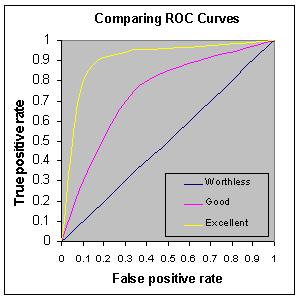
\includegraphics[width = (\textwidth)/2]{roccomp.jpg}
  \caption{Example of a ROC curve}
  \label{fig:ROC}
\end{figure}


With the research conducted in this section an approach of using several metrics seems to be the best choice to evaluate the research artefact. Some of these could be ROC curves and MAE. Specific metrics that will be used will be further researched and decided upon at a later date.\\ \\

%\cite{6608492}

\section{Conclusion}
In conclusion the literature explored in this chapter has helped to guide the development of the research artefact. Neural Networks was the algorithm chosen to train the model on. Data scraping was looked into further for collecting data to build a data set, but was not used more on this can be found in the data set chapter. Evaluation metrics used to aid in the evaluation of the model came from within the literature, confusion metrics were printed for each implementation of the model so a quick analysis could be done to compare the latest iteration to the previous. 